\newpage
\section{先行研究の内容}
%%%%%%%%%%%%%%%%%%%%%%%%%%%%%%%%%%%%%%%%%%%%%%%%%%%%%%%%%
\subsection{McKibben型空気圧人工筋肉アクチュエータ(MPA)}
% ・今のとこは先輩のやつを真似ただけ.
MPAはシリコンゴムチューブをナイロンメッシュで覆うことで構成されており(図\ref{fig:MPA}\subref{fig:Structure}),両端に栓をするシンプルな構造である.
これに圧縮した空気を印加することでシリコンゴムチューブが膨張しメッシュによる自身の軸方向への張力が発生するアクチュエータである(図\ref{fig:MPA}\subref{fig:move}).
高出力かつ素材自体も軽量で,物理的柔軟性による高い弾性力を持つという利点があり,筋肉の代用として生物を模したロボットやリハビリなどに用いられる.
%%%%%%%%%%%%%%%%%%%%%%%%%%%%%%%%%%%%%%%%%%%%%%%%%%%%%%%%%
\begin{figure}[b]
  %
  \begin{minipage}{0.49\columnwidth}
    \vspace{4mm}
    \centering
    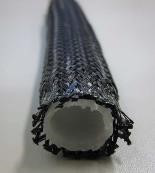
\includegraphics[scale=1]{image/MPA_kousei.png}
    \vspace{3mm}
    \subcaption{MPA断面図}
    \label{fig:Structure}
  \end{minipage}
  %
  \begin{minipage}{0.49\columnwidth}
    \vspace{10mm}
    \centering
    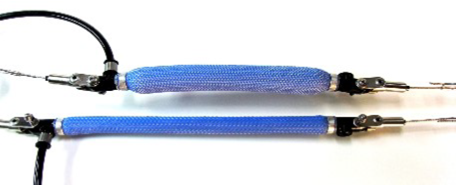
\includegraphics[scale=.8]{image/MPA_dousa.png}
    \vspace{10mm}
    \subcaption{MPA外観および動作の様子}
    \label{fig:move}
  \end{minipage}
  %
  \caption{McKibben型空気圧人工筋(MPA)の構成および外観\cite{中西大輔2020}}
  \label{fig:MPA}
\end{figure}
%%%%%%%%%%%%%%%%%%%%%%%%%%%%%%%%%%%%%%%%%%%%%%%%%%%%%%%%%
\subsection{細径MPA}
% ・脇本修一の論文を参考に細径MPAの冗長性,従来のMPAとの比較などについて説明,φ3のMPAの写真
本研究で用いる細径のMPAについて説明する.図\ref{fig:campare}に本研究で開発に成功した外径5 mmと3 mmの細径MPAと外径12 mmの従来のMPAを示す.
細径化には下記のような利点があると考えられている\cite{wakimoto}\cite{1390282680917523328}.
\begin{enumerate}
  \item 非常にしなやかな人工筋となり座屈することなく任意形状での配置や集積が可能
  \item 集積化により収縮量を増大させることが可能
  \item 集積化により冗長性を持ちシステムの安全性が向上
\end{enumerate}
MPAの収縮力は断面積に比例するため,細径MPAは従来のものに比べると発生する張力は小さいものの,細くしなやかであり任意形状での配置や集積化が可能である.
生体筋と柔らかさや動作が似ていることから,紡錘状に集積し筋骨格系ロボット(図\ref{fig:saikei}\subref{fig:kin})へ応用したり,生物模倣ロボットとしてタコ腕模倣メカニズム(図\ref{fig:saikei}\subref{fig:tako})も開発されており,曲げ動作やねじり動作を実現している\cite{森和也2014}.
%%%%画像置き場%%%%%%%%%%%%%%%%%%%%%%%%%%%%%%%%%%%%%%%%%%%%
\begin{figure}[t]
  \centering
  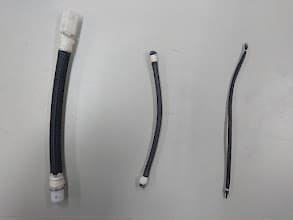
\includegraphics[scale=0.7]{image/hikaku.jpg}
  \caption{MPAの外径の比較(左から12,5,3 mm)}
  \label{fig:campare}
\end{figure}
%
\begin{figure}
  %
  \begin{minipage}{0.5\columnwidth}
    \centering  
    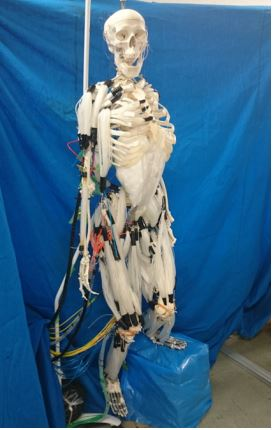
\includegraphics[scale=0.5]{image/kinkokkaku.JPG}
    \subcaption{筋骨格系ロボット\cite{森田隆介2016}}
    \label{fig:kin}
  \end{minipage}
  %
  \begin{minipage}{0.5\columnwidth}
    \centering
    \vspace{5mm}
    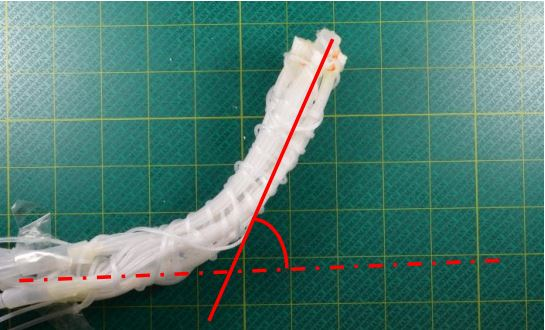
\includegraphics[scale=0.57]{image/takoJPG.JPG}
    \subcaption{タコ腕模倣メカニズム\cite{森和也2014}}
    \label{fig:tako}
  \end{minipage}
  %
  \caption{細径空圧筋を用いたロボット}
  \label{fig:saikei}
\end{figure}
%%
\begin{figure}[t]
  \centering
  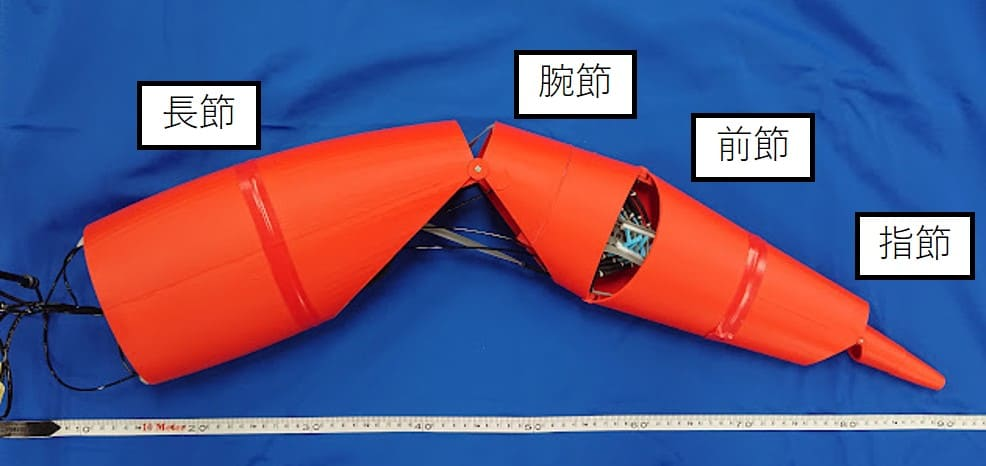
\includegraphics[scale=0.3]{image/robot_scale.JPG}
  \vspace{3mm}
  \caption{先行研究で作製された歩脚ロボット\cite{hasegawa}}
  \label{fig:senkoukenkyuu}
\end{figure}
  %
\begin{figure}[t]
  \centering
  \vspace{3mm}
  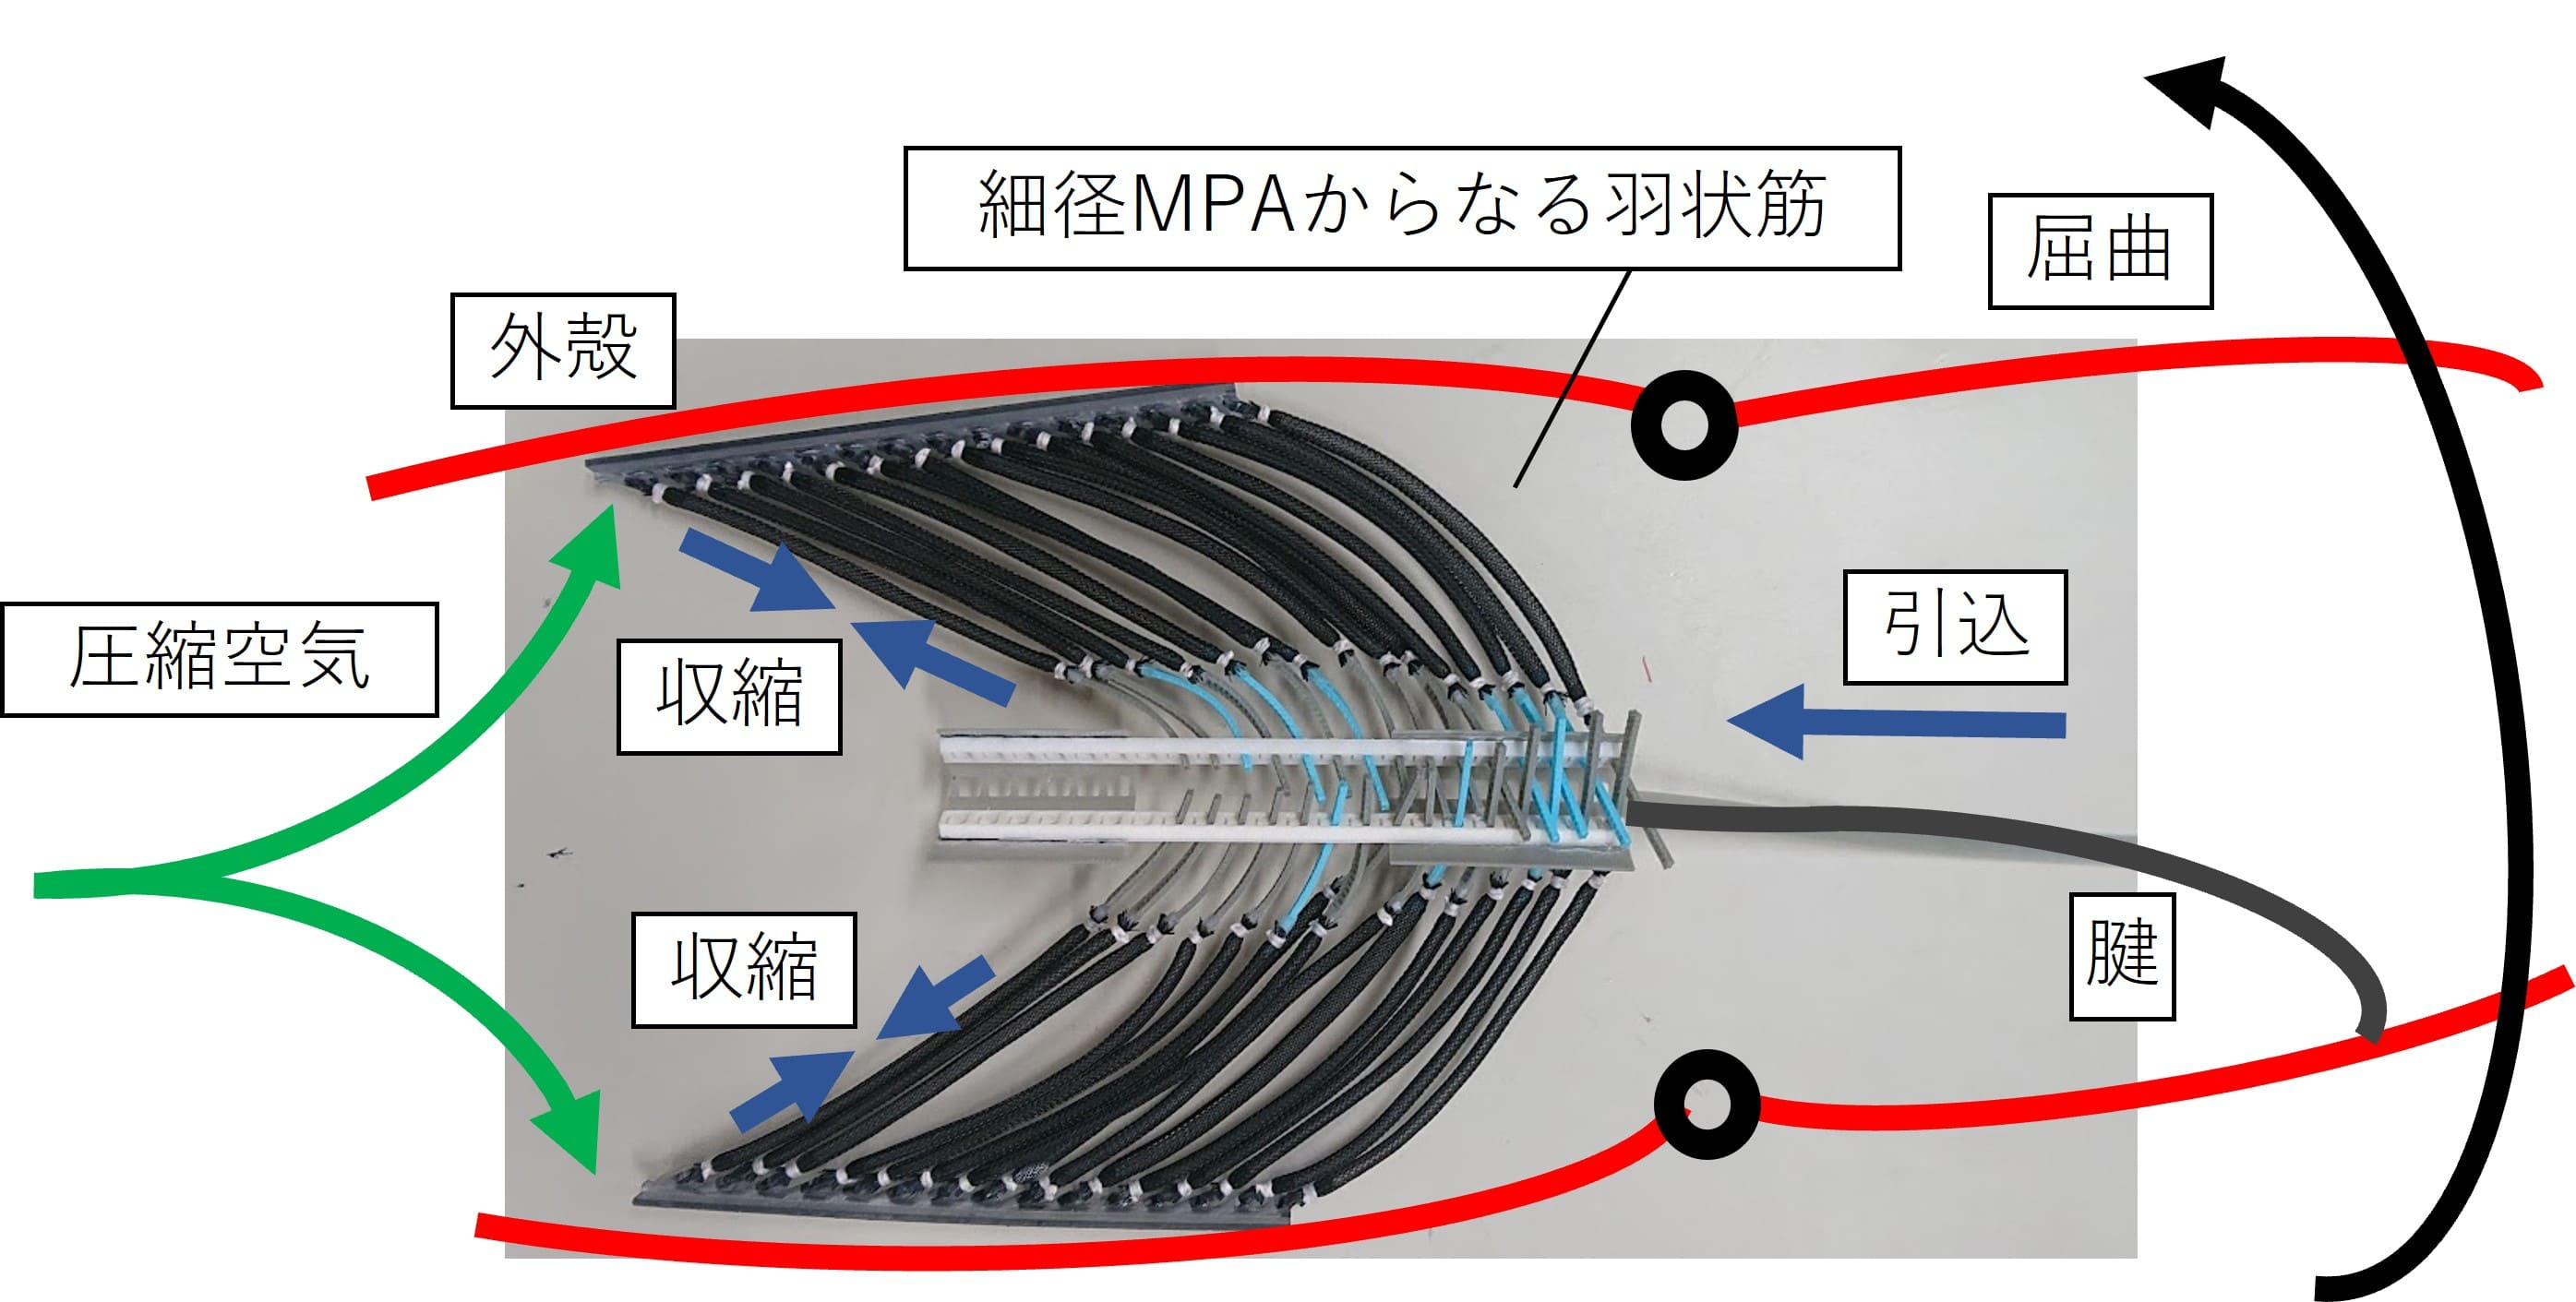
\includegraphics[scale=0.14]{image/mosiki.JPG}
  \caption{先行研究で開発された羽状筋\cite{hasegawa}}
  \label{fig:ujyoukin}
\end{figure}
%%
\begin{figure}[tbp]
  \begin{minipage}{1\hsize}
    \centering
    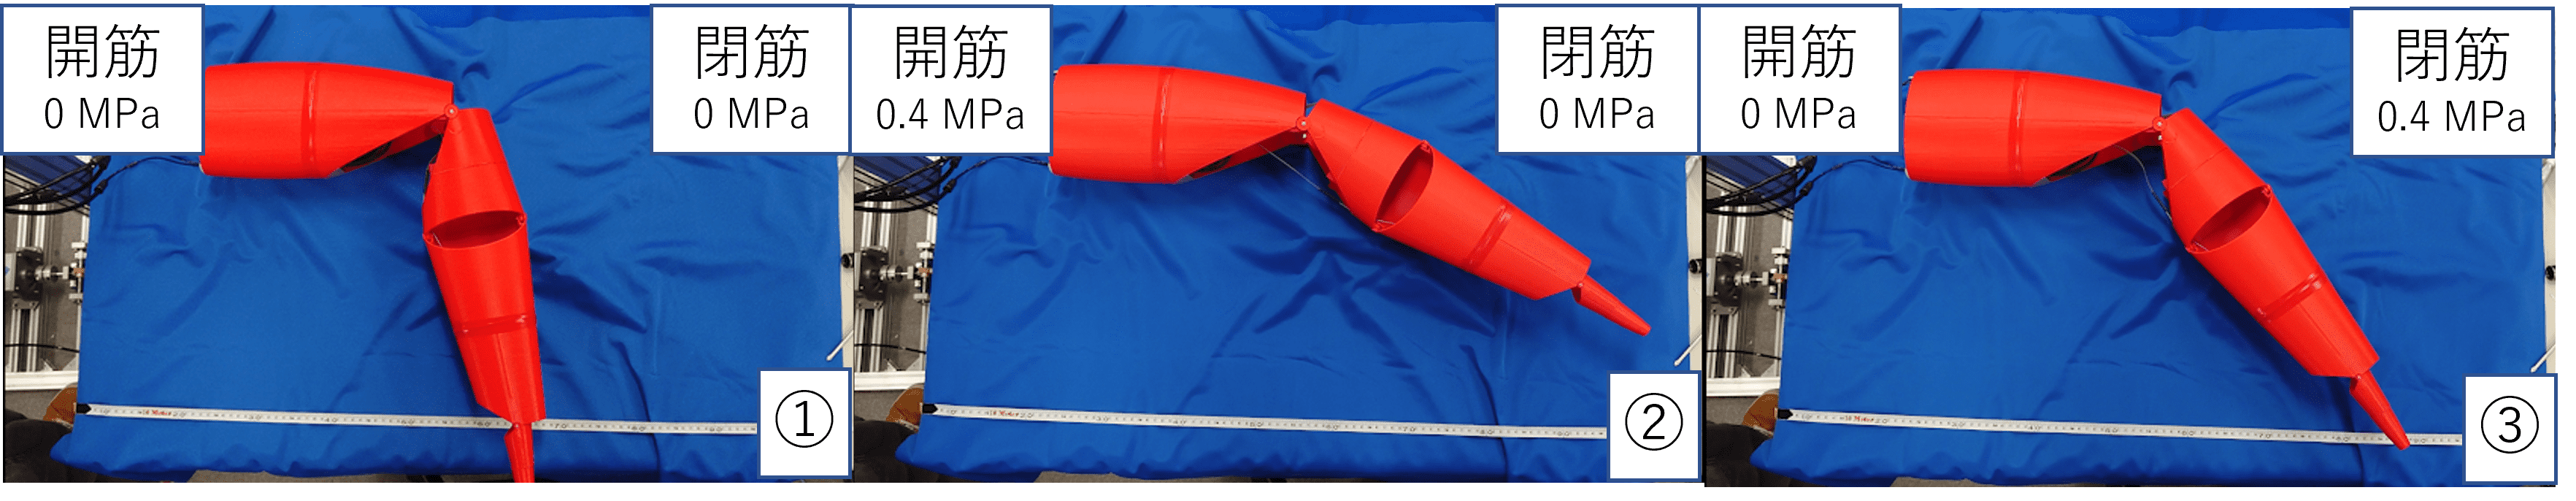
\includegraphics[scale=0.12]{image/move1all.png}
    \subcaption{長節-腕節間の動作\cite{hasegawa}}
    \label{fig:move1}
  \end{minipage}
  %
  \begin{minipage}{1\hsize}
    \centering
    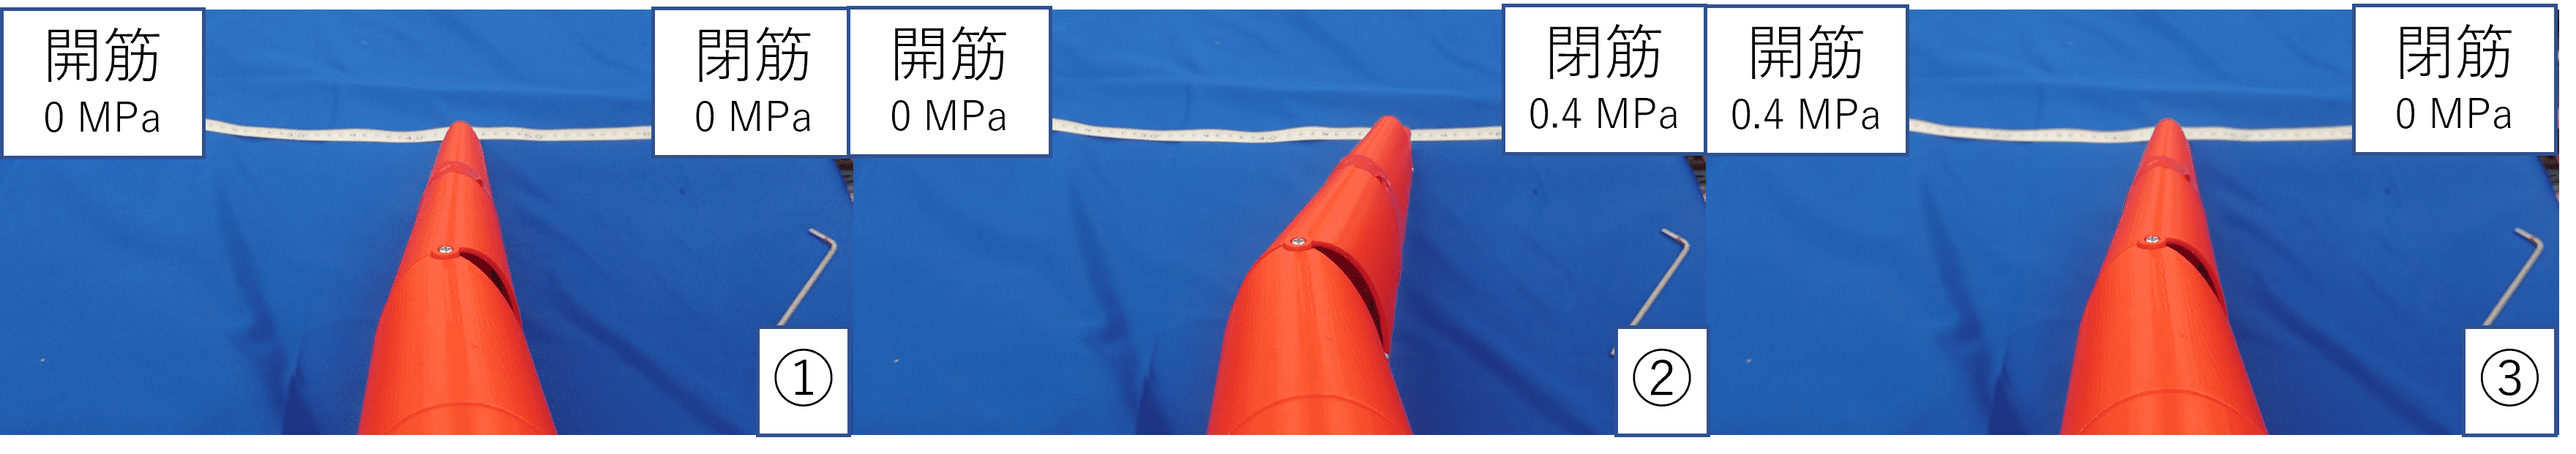
\includegraphics[scale=0.12]{image/move2all.png}
    \subcaption{腕節-前節間の動作\cite{hasegawa}}
    \label{fig:move2}
  \end{minipage}
%
  \caption{動作実験}
  \label{fig:movea12}
\end{figure}
%
%%%%%%%%%%%%%%%%%%%%%%%%%%%%%%%%%%%%%%%%%%%%%%%%%%%%%%%%%
\subsection{先行研究の成果と課題}
先行研究では図\ref{fig:senkoukenkyuu}\cite{hasegawa}のような歩脚ロボットの作製に成功した.このロボットでは図\ref{fig:ujyoukin}のように細径MPAを用いて蟹の羽のような筋肉である羽状筋と呼ばれる筋肉を再現することができた\cite{hasegawa}.
このロボットで動作実験を行い図\ref{fig:movea12}のように開閉動作をすることを確認することができた.
しかし,以下のような課題点が見つかった\cite{hasegawa}
\begin{enumerate}
  \item 細径MPAの作製方法が煩雑で時間がかかってしまい,成功させるのに技術が必要
  \item 細径MPAの収縮性能が低くて,腱が少ししか引き込めなかった
  \item 細径MPAの根元部分の角度が固定されていて,腱を引き込む妨げになっていた
\end{enumerate}
そこで本研究では,上記のような先行研究で見つかった課題点を解決した歩脚ロボットの作製に取り組む.
